\documentclass[tikz,border=8pt]{standalone}
% Shared look for every TikZ diagram. Load with \input{../../tools/tikz-style.tex}
\usepackage[T1]{fontenc}
\usepackage{lmodern}
\renewcommand{\sfdefault}{lmr}  % diagrams use the same serif as the text
\usetikzlibrary{arrows.meta, positioning, shapes.geometric, calc, fit, backgrounds}
\definecolor{cblue}{HTML}{4C78A8}
\definecolor{corange}{HTML}{F58518}
\definecolor{cgreen}{HTML}{54A24B}
\definecolor{cred}{HTML}{E45756}
\definecolor{cpurple}{HTML}{B279A2}
\definecolor{cgrey}{HTML}{6B6B6B}
\tikzset{
  every picture/.style={font=\sffamily, line width=1.2pt},
  box/.style={draw=#1, fill=#1!12, rounded corners=4pt, align=center, inner sep=7pt, minimum height=1.1cm},
  box/.default=cgrey,
  arrow/.style={-{Stealth[length=3mm]}, draw=cgrey, line width=1.4pt},
  title/.style={font=\sffamily\bfseries\Large},
  note/.style={font=\sffamily\small, text=cgrey, align=center},
}
\AtBeginDocument{\hyphenpenalty=10000 \exhyphenpenalty=10000}

\begin{document}
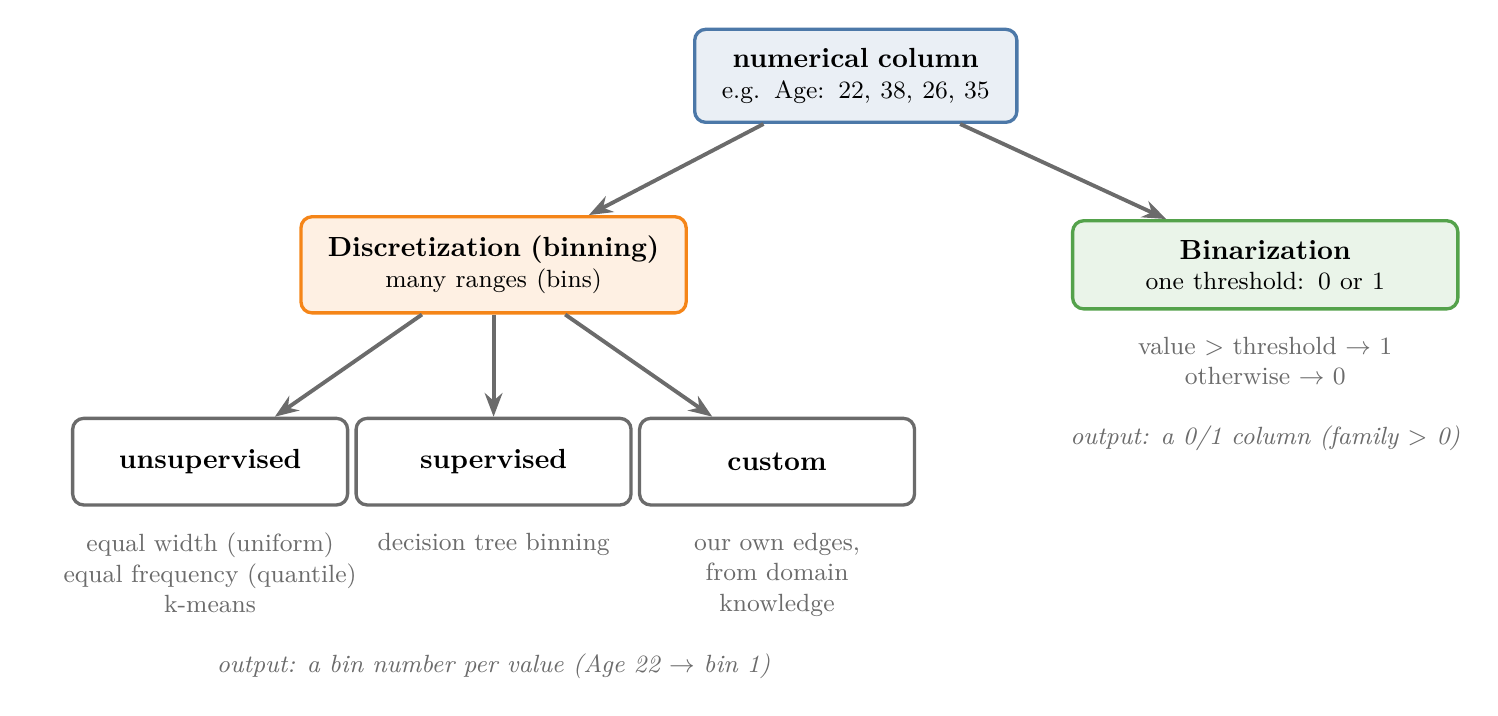
\begin{tikzpicture}
  \node[box=cblue, text width=3.6cm] (in) at (0,0) {\textbf{numerical column}\\[-1pt]\small e.g. Age: 22, 38, 26, 35};
  % two techniques
  \node[box=corange, text width=4.4cm] (disc) at (-4.6,-2.4) {\textbf{Discretization (binning)}\\[-1pt]\small many ranges (bins)};
  \node[box=cgreen, text width=4.4cm] (bin) at (5.2,-2.4) {\textbf{Binarization}\\[-1pt]\small one threshold: 0 or 1};
  \draw[arrow] (in) -- (disc);
  \draw[arrow] (in) -- (bin);
  % kinds of binning
  \node[box=cgrey, fill=white, text width=3.0cm] (uns) at (-8.2,-4.9) {\textbf{unsupervised}};
  \node[box=cgrey, fill=white, text width=3.0cm] (sup) at (-4.6,-4.9) {\textbf{supervised}};
  \node[box=cgrey, fill=white, text width=3.0cm] (cus) at (-1.0,-4.9) {\textbf{custom}};
  \foreach \k in {uns, sup, cus} \draw[arrow] (disc) -- (\k);
  \node[note, below=0.2cm of uns, text width=4.4cm] {equal width (uniform)\\ equal frequency (quantile)\\ k-means};
  \node[note, below=0.2cm of sup, text width=3.0cm] {decision tree binning};
  \node[note, below=0.2cm of cus, text width=3.0cm] {our own edges,\\ from domain knowledge};
  \node[note, below=0.2cm of bin, text width=4.6cm] {value $>$ threshold $\rightarrow$ 1\\ otherwise $\rightarrow$ 0};
  % outputs
  \node[note, font=\sffamily\small\itshape] at (-4.6,-7.5) {output: a bin number per value (Age 22 $\rightarrow$ bin 1)};
  \node[note, font=\sffamily\small\itshape] at (5.2,-4.6) {output: a 0/1 column (family $>$ 0)};
\end{tikzpicture}
\end{document}
